%-------------------------------------------------------------------------------
\subsection{Calcul différentiel}
%-------------------------------------------------------------------------------

\todo{Voir L3 Bio SU : TD1, exercice 2}

%-------------------------------------------------------------------------------
\subsection{Systèmes dynamiques en dimension 1}
%-------------------------------------------------------------------------------

\todo{Voir L3 Bio SU : TD2, exercice 1}

\exemple{[Exercice 2, TD2, L2 Bio SU]
  On considère le système
  $$
  \dot y = - y^3 + 7 y^2 - 14 y + 8.
  $$
  Ses points stationnaires sont les racines du polynôme $P(y) = - y^3 + 7 y^2 - 14 y + 8$, donc $y_1 = 1$ fait partie, donc
  $$
  P(y) = (y-1) (-y^2 + 6y + 8),
  $$
  et les deux racines de $-y^2 + 6y + 8$ sont $2$ et $4$. Les points stationnaires du système sont donc 
  $$
  y_1 = 1, \qquad y_2 = 2, \qquad y_3 = 4.
  $$
  Leur stabilité est donné par la dérivée de $P$:
  $$
  P'(y) = -3y^2 + 14 y - 14,
  $$
  soit
  $$
  P'(y_1) = -3, \qquad P'(y_2) = 2, \qquad P'(y_3) = -6.
  $$
  $y_1$ et $y_3$ sont donc des équilibres stables, et $y_2$ un équilibre instable.
  $$
  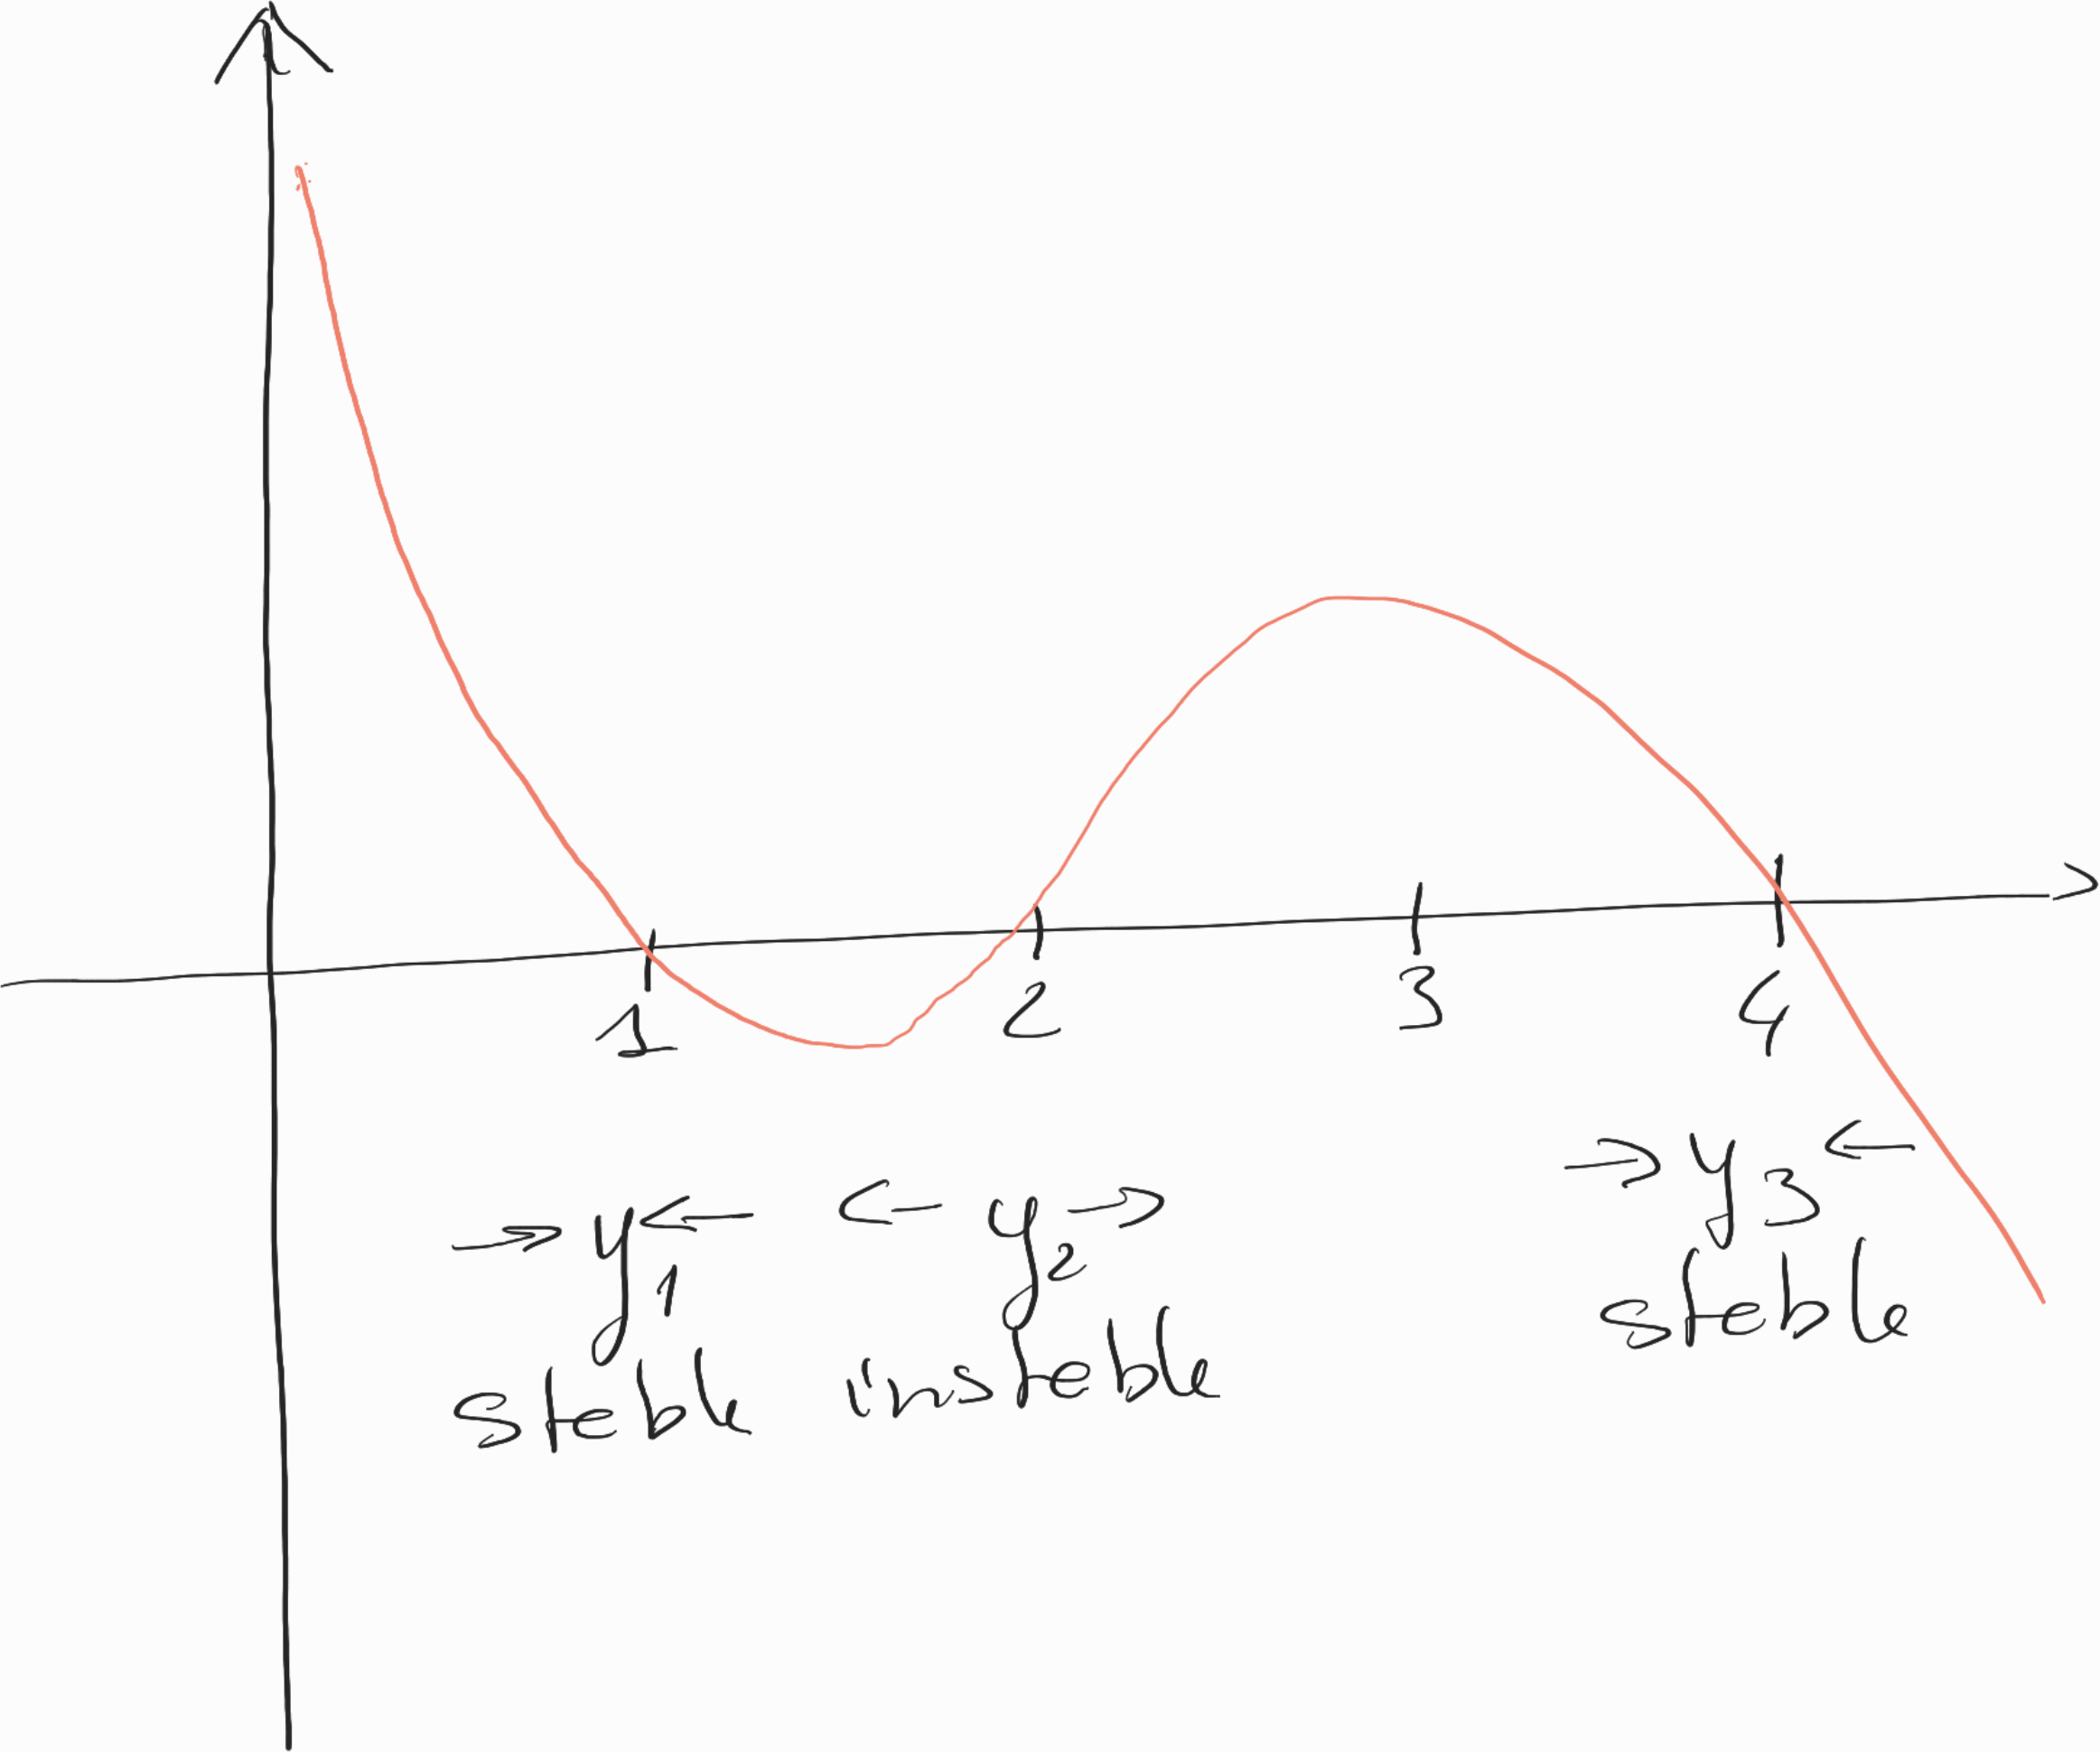
\includegraphics[width=.5\textwidth]{TD-SUbioL3-TD2Exo2}
  $$
}

%-------------------------------------------------------------------------------
\subsection{Systèmes dynamiques en dimension 2}
%-------------------------------------------------------------------------------

%-------------------------------------------------------------------------------
\paragraph{Système dynamique linéaire.} 
On considère le système dynamique suivant
$$
\left\{\begin{array}{rcl}
        \dot x & = & -a_1 x + b_1 y + c_1 \\ 
        \dot y & = & -a_2 x + b_2 y + c_2
        \end{array}\right.
$$
où tous les coefficients constants sont strictement positifs.
\begin{enumerate}
  \item À quelle condition y a-t-il un unique équilibre ? Lorsque c’est le cas, à quelle condition est-il stable ?
  \item Lorsqu’il n’existe pas d’équilibre unique, représenter les deux isoclines (c'est à dire les ensemble de points ou s'annule $\dot x$ d'une part et $\dot y$ d'autre part). Y a-t-il une infinité d’équilibres ou aucun équilibre ?
  \item Représenter les orbites dans le plan de phase.
\end{enumerate}

\solution{\todo{}}

%-------------------------------------------------------------------------------
\paragraph{Système dynamique quadratique.} \label{SystDyn-Quadratique}
On considère le système dynamique d’activation réciproque suivant avec compétition intraspécifique
$$
%   \SR{
%   \left\{\begin{array}{rcl}
%          \dot x & = & r y - cx^2 \\ 
%          \dot y & = & r x - cy^2 
%          \end{array}\right.
%   }{
\left\{\begin{array}{rcl}
        \dot x & = & a y - x^2 \\ 
        \dot y & = & a x - y^2 
        \end{array}\right.
%   }
$$
%   où $r$ et $c$ sont deux constantes strictement positives.
où $a$ est une constante strictement positive.
\begin{enumerate}
  \item Donner la valeur $(x^*, y^*)$ de l’unique équilibre non trivial\footnote{'Trivial' signifie à la fois évident et sans intérêt. En l'occurrence, le point d'équilibre trivial est le point $(0, 0)$.} de ce système dans le quadrant positif. Quel est l’autre équilibre ?
  \solution{$(x=0, y=0)$ est le point d'équilibre trivial. L'autre point d'équilibre s'obtient en résolvant
  $$
  \left\{\begin{array}{rcl}
          a y & = & x^2 \\
          a x & = & y^2
        \end{array}\right.
  \quad \Leftrightarrow \quad
  \left\{\begin{array}{rcl}
          y & = & x^2 / a \\
          a x & = & x^4 / a^2
        \end{array}\right.
  \quad \Leftrightarrow \quad
  \left\{\begin{array}{rcl}
          y & = & x^2 / a \\
          a^3 & = & x^3
        \end{array}\right.
  \quad \Leftrightarrow \quad
  x^* = y^* = a
  $$}
  \item Donner la nature de chacun de ces deux équilibres.
  \solution{En notant
  $$
  F(x, y) = \left[\begin{array}{rcl} 
                    F_1(x, y) & = & ay - x^2 \\
                    F_2(x, y) & = & ax - y^2
                  \end{array}\right],
  $$
  on a
  $$
  J_{(x, y)} F = \left[\begin{array}{cc}-2x & a \\ a & -2y\end{array}\right].
  $$
  \begin{description}
    \item[Point $(0, 0)$:] on a
    $$
    J_{(0, 0)} F = \left[\begin{array}{cc}0 & a \\ a & 0\end{array}\right]
    \quad \Rightarrow \quad
    P(\lambda) = \lambda^2 - a^2
    $$
    qui s'annule pour $\lambda = \pm a$. Des vecteurs associés à $a$ et $-a$ sont, respectivement $[1 \; 1]^\top$ et $[-1 \; 1]^\top$. \\
    $(0, 0)$ est un équilibre instable dans la direction de la première bissectrice et stable dans celle de la seconde.
    \item[Point $(a, a)$:] an a
    $$
    J_{(0, 0)} F = \left[\begin{array}{cc}-2a & a \\ a & -2a\end{array}\right]
    \quad \Rightarrow \quad
    P(\lambda) = \lambda^2 - a^2
    \quad \Rightarrow \quad
    P(\lambda) = \lambda^2 - 4 a \lambda + 3 a^2
    $$
    qui s'annule pour $\lambda = -a$ et $\lambda = -3a $. \\
    $(a, a)$ est donc un équilibre stable.
  \end{description}
  }
  \item Que se passe-t-il si $x(0) = y(0) > 0$ ? Représenter l’allure des trajectoires dans le plan de phase. 
  \solution{
  On peut remarquer que 
  $$
  \{\dot x = 0\} \Leftrightarrow \{y = x^2/a\}, \qquad
  \{\dot y = 0\} \Leftrightarrow \{y = \sqrt{a x}\}
  $$
  $$
  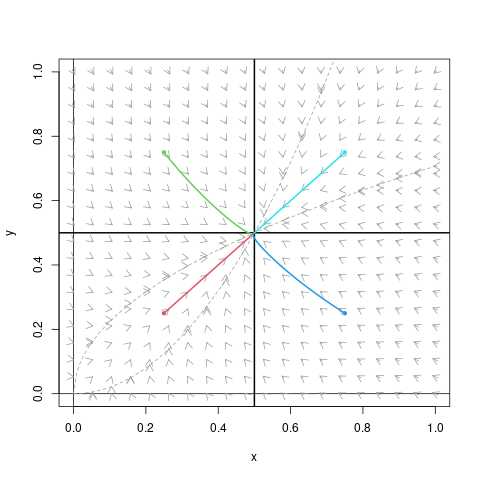
\includegraphics[width=.45\textwidth, trim=0 10 20 20, clip=]{ActivationReciproque}
  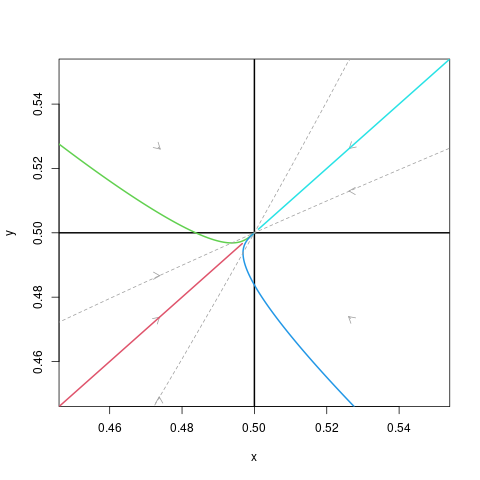
\includegraphics[width=.45\textwidth, trim=0 10 20 20, clip=]{ActivationReciproque-zoom}
  $$
  Toutes les trajectoires convergent vers $(a, a)$.
  \begin{description}
    \item[$(x_0 < a, y_0 < a)$:] la trajectoire converge directement vers $(a, a)$.
    \item[$(x_0 < a, y_0 > a)$:] la trajectoire franchit l'axe $y = a$ avant de revenir en $(a, a$.
    \item[$(x_0 > a, y_0 > a)$:] la trajectoire converge directement vers $(a, a)$.
    \item[$(x_0 > a, y_0 < a)$:] la trajectoire franchit l'axe $x = a$ avant de revenir en $(a, a)$.
  \end{description}
  }
\end{enumerate}


%-------------------------------------------------------------------------------
\begin{exercise}[Cycle limite] 
  \todo{Voir exemple 1, p 195, Perko, 2001}
\end{exercise}

